% ============================================================
%  第六章  无人机检测模块设计
% ============================================================
\section{无人机检测模块设计}

本模块运行于 5001 端口，负责“把视频变成轨迹”：输入左右目两路视频，逐帧检测无人机目标，通过双目三角测量恢复三维位置，再以多目标跟踪串成连续轨迹，最终写入与重建模块共享的数据目录。

\subsection{模块组成与数据流}

模块代码位于 \file{trajectory_recognition/}，由四个算法组件、两个服务组件和接口/表现层组成。数据在模块内的流转如图~\ref{fig:detflow} 所示。

\begin{figure}[H]
\centering
\begin{tikzpicture}[node distance=7mm and 9mm]
\node[term] (v) {左目 / 右目视频};
\node[proc, below=6mm of v, text width=40mm] (vp) {视频预处理\\抽帧 · 缩放 · 时间戳};
\node[proc, below left=10mm and 20mm of vp, text width=32mm] (d1) {左目 YOLO 推理};
\node[proc, below right=10mm and 20mm of vp, text width=32mm] (d2) {右目 YOLO 推理};
\node[proc, below=14mm of vp, text width=44mm] (mt) {左目多目标跟踪\\ByteTrack / BoT-SORT};
\node[proc, below=6mm of mt, text width=44mm] (sm) {跨目匹配\\类别 + 行对齐 + 视差 + 尺寸};
\node[proc, below=6mm of sm, text width=44mm] (tri) {三角测量\\$Z=fB/d$};
\node[proc, below=6mm of tri, text width=44mm] (wd) {世界坐标变换\\$Y$ 翻转 + 旋转 + 平移};
\node[proc, below=6mm of wd, text width=44mm] (as) {3D 点关联\\按 IoU 挂到 Track};
\node[data, below=6mm of as, text width=40mm] (out) {data/fact/\{平台\}.npz};
\draw[arr] (v) -- (vp);
\draw[arr] (vp.south) -- (d1.north);
\draw[arr] (vp.south) -- (d2.north);
\draw[arr] (d1.south) |- (mt.west);
\draw[arr] (d2.south) -- ++(0,-0.25) -| (sm.east);
\draw[arr] (mt) -- (sm);
\draw[arr] (sm) -- (tri);
\draw[arr] (tri) -- (wd);
\draw[arr] (wd) -- (as);
\draw[arr] (as) -- (out);
\end{tikzpicture}
\caption{检测模块数据流}
\label{fig:detflow}
\end{figure}

四个算法组件与两个服务组件的职责如表~\ref{tab:detcomp} 所示。

\begin{table}[H]
\centering
\caption{检测模块组件职责}
\label{tab:detcomp}
\small
\begin{tabularx}{\linewidth}{@{}>{\heiti\scriptsize}p{2.6cm}>{\raggedright\ttfamily\scriptsize}p{4.4cm}>{\raggedright\arraybackslash}X@{}}
\toprule
组件 & 源文件 & 职责 \\
\midrule
视频预处理 & detection/preprocess.py & 打开文件/流/摄像头，按间隔抽帧，计算帧号与时间戳 \\
检测引擎 & detection/engine.py & 加载 YOLO 权重，单帧推理，类别过滤与置信度排序 \\
多目标跟踪 & detection/tracker.py & 维护 Track 集合与 ID，记录 2D/3D 轨迹点 \\
双目立体视觉 & detection/stereo.py & 焦距推算、三角测量、跨目匹配 \\
检测服务 & services/detection\_service.py & 会话状态机、后台线程、预览帧缓存、坐标变换 \\
数据桥接 & services/data\_bridge.py & 轨迹合并写盘、旧文件备份、通知重建模块 \\
\bottomrule
\end{tabularx}
\end{table}

\subsection{视频预处理}

\code{VideoProcessor} 以生成器方式逐帧产出 \code{Frame} 对象（图像、帧号、时间戳），避免一次性把整个视频读入内存。其设计要点如下：

\begin{itemize}
  \item \term{多源统一}：\code{cv2.VideoCapture} 同时支持本地文件、RTSP/HTTP 流与 USB 摄像头，接口层无需区分；
  \item \term{抽帧}：\code{frame_interval} 控制每隔多少帧处理一次，默认 3；时间戳仍按原始帧号除以帧率计算，保证与真实时间一致；
  \item \term{元信息先行}：\code{get_video_info()} 只读文件头即可获得帧率、总帧数、分辨率与时长，用于进度计算，避免遍历全部帧；
  \item \term{资源释放}：生成器在 \code{finally} 中调用 \code{release()}，即使中途异常也不会泄漏视频句柄。
\end{itemize}

\subsection{YOLO 检测引擎}

\code{YOLODetector} 对 ultralytics 做了一层薄封装，把“模型加载”与“推理”分离，并统一输出 \code{Detection} 数据类。

\subsubsection{延迟加载与设备适配}

权重在首次推理时才加载（\code{model} 属性内部判空），因此“打开页面但不检测”的启动开销接近于零，这对桌面一体化应用很重要。设备字符串做两级规范化：\code{auto} 依据 \code{torch.cuda.is_available()} 决定；\code{cuda:N} 转换为 ultralytics 接受的 \code{N}。

\subsubsection{推理与过滤}

推理参数包括置信度阈值、NMS 阈值、输入尺寸与设备。推理后按 \code{target_classes} 过滤类别，并按置信度降序排序，使后续匹配优先处理高置信目标。由于 COCO 数据集中没有 \code{drone} 类，系统默认关注 \code{bird}(14)、\code{airplane}(4) 作为近似，实际部署时应使用自训练的无人机模型（类别 0）。

\subsubsection{预热}

首次推理需完成 CUDA 上下文初始化与算子编译，耗时可达数秒。\code{warmup()} 用零矩阵做一次前向，把这部分开销前移到“开始检测”之前，避免首帧卡顿。

\subsection{模型训练与评估}

检测精度取决于自定义模型。项目提供了独立的训练脚本 \file{train/yolotrain/train.py}，在 ultralytics 训练流程之上增加了训练曲线绘制、指标汇总与结果对比功能。

\subsubsection{训练配置}

本次训练采用 YOLOv8n 作为骨干网络，在自建无人机数据集上训练，主要参数如表~\ref{tab:trainargs} 所示。

\begin{table}[H]
\centering
\caption{YOLO 无人机检测模型训练参数}
\label{tab:trainargs}
\small
\begin{tabularx}{\linewidth}{@{}>{\heiti}p{3.4cm}p{3.0cm}X@{}}
\toprule
参数 & 取值 & 说明 \\
\midrule
基础权重 & yolov8n.pt & 轻量模型，便于边缘部署 \\
训练轮数 & 120（实际 95） & 早停耐心 20 轮，第 75 轮后指标不再提升 \\
输入尺寸 & 1280$\times$1280 & 高分辨率以保留远距离小目标细节 \\
批次大小 & 16 & CPU 训练下的显存/内存折中 \\
优化器 & AdamW，初始学习率 0.01 & 余弦退火，最后 10 轮关闭 Mosaic \\
数据增强 & Mosaic 1.0、HSV、随机缩放 0.3、水平翻转 0.5、随机旋转 15° & 上下翻转关闭（天空在上） \\
训练设备 & CPU & 无可用 GPU 时的兜底方案 \\
\bottomrule
\end{tabularx}
\end{table}

\subsubsection{训练结果}

训练过程的损失与指标曲线如图~\ref{fig:yolodash} 所示。三类损失（box、cls、dfl）均平稳下降，验证集损失在后期趋于平缓，未出现明显过拟合。

\begin{figure}[H]
\centering
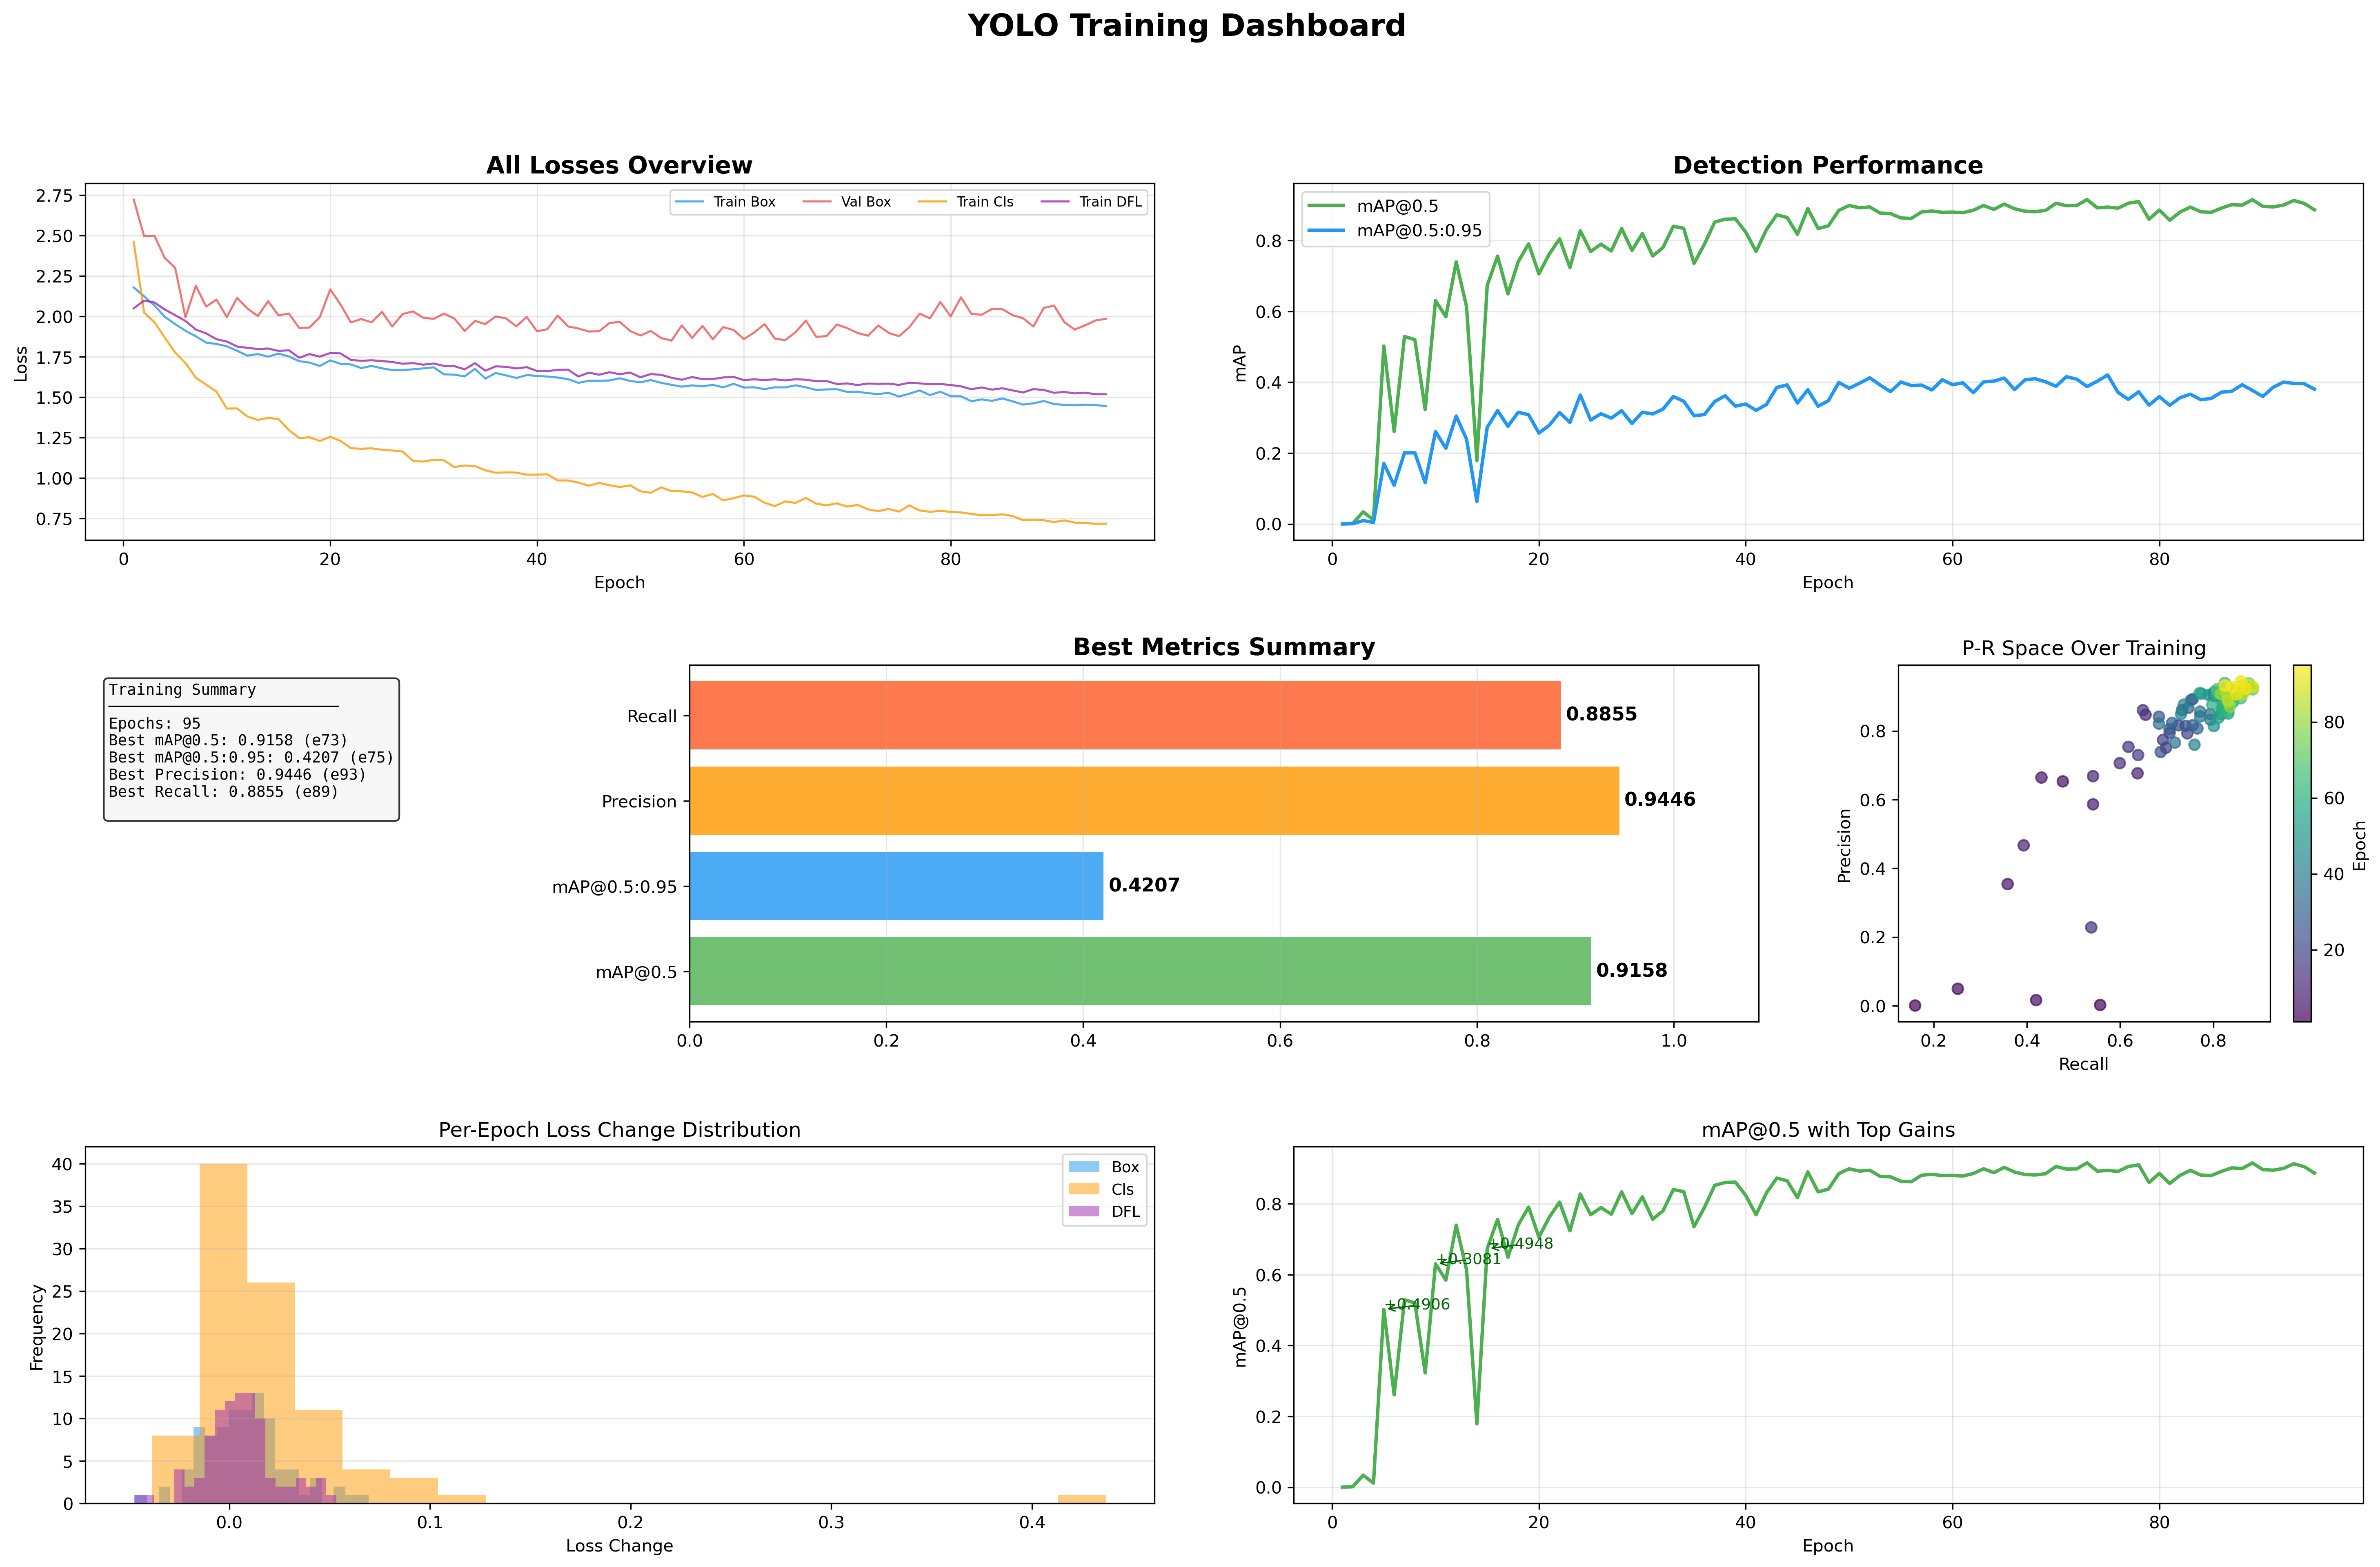
\includegraphics[width=0.92\linewidth]{figures/yolo/04_dashboard.png}
\caption{YOLO 训练过程综合仪表盘（损失、精度、召回率与 mAP）}
\label{fig:yolodash}
\end{figure}

第 95 轮（末轮）的验证指标为：精确率 0.928、召回率 0.840、mAP@0.5 为 0.905、mAP@0.5:0.95 为 0.396，全程最佳 mAP@0.5 达到 \textbf{0.916}。

从统计结果看，\textbf{精确率 0.928 与召回率 0.840 均较为优秀}：高精确率意味着报警结果可信、值班人员无需在大量误报中筛选，高召回率意味着绝大多数闯入目标都能被及时发现。两项指标同时保持在较高水平，说明模型在“不误报”与“不漏报”之间取得了良好平衡，能够满足低空无人机监测的使用要求；配合双目三角测量与多目标跟踪后，系统可在连续视频中稳定输出三维轨迹。



\begin{figure}[H]
\centering
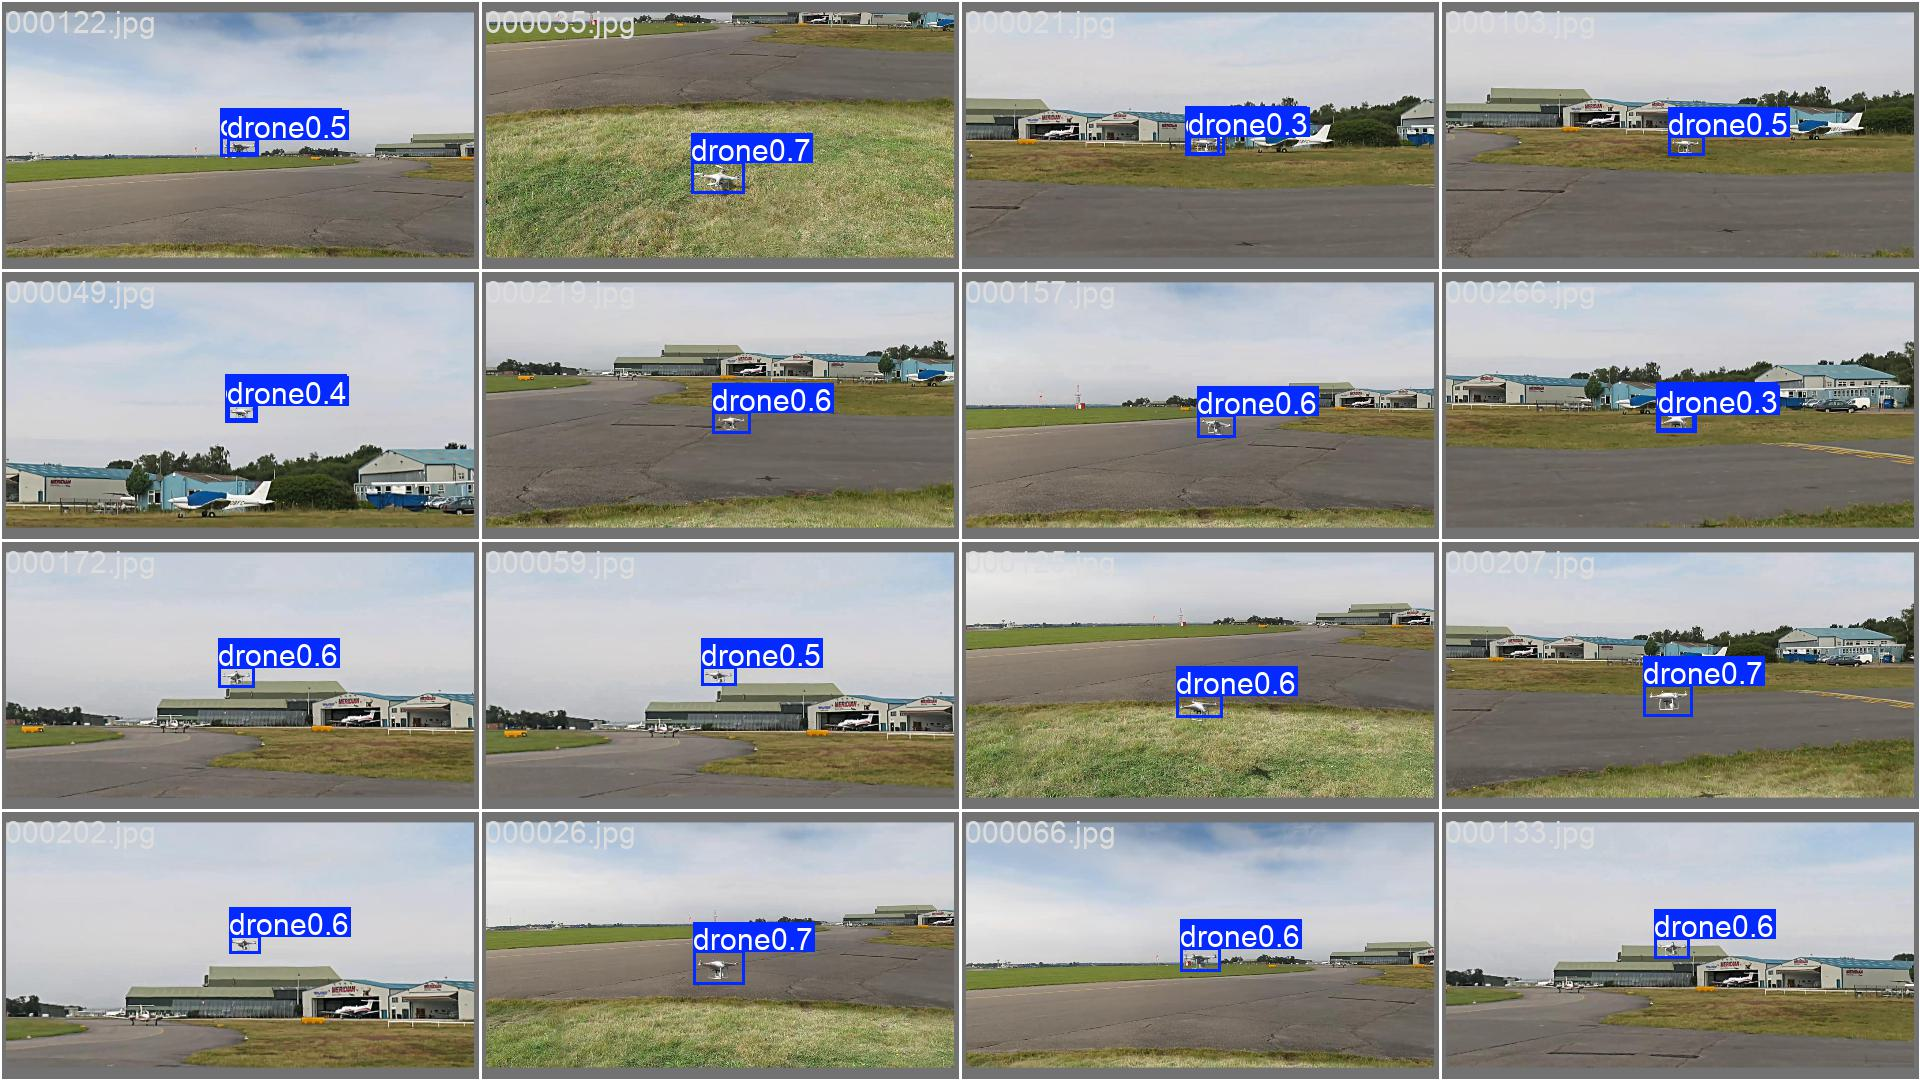
\includegraphics[width=0.78\linewidth]{figures/yolo/val_batch0_pred.jpg}
\caption{验证集检测结果示例（机场场景下的无人机目标）}
\label{fig:yolopred}
\end{figure}

从图~\ref{fig:yolopred} 可以看到，目标在画面中仅占数十像素，属于典型小目标检测场景；模型在草坪、跑道、机库等复杂背景下均能给出稳定框选，置信度集中在 0.3--0.7 之间，说明模型对该数据集的输出稳定、可信，与上述精确率与召回率的统计结果一致。

图~\ref{fig:yolopr} 给出验证集的 Precision--Recall 曲线：曲线整体靠近右上角，在不同置信度阈值下都能同时保持较高的精确率与召回率，说明模型对阈值选择不敏感，具备良好的部署适应性。

\begin{figure}[H]
\centering
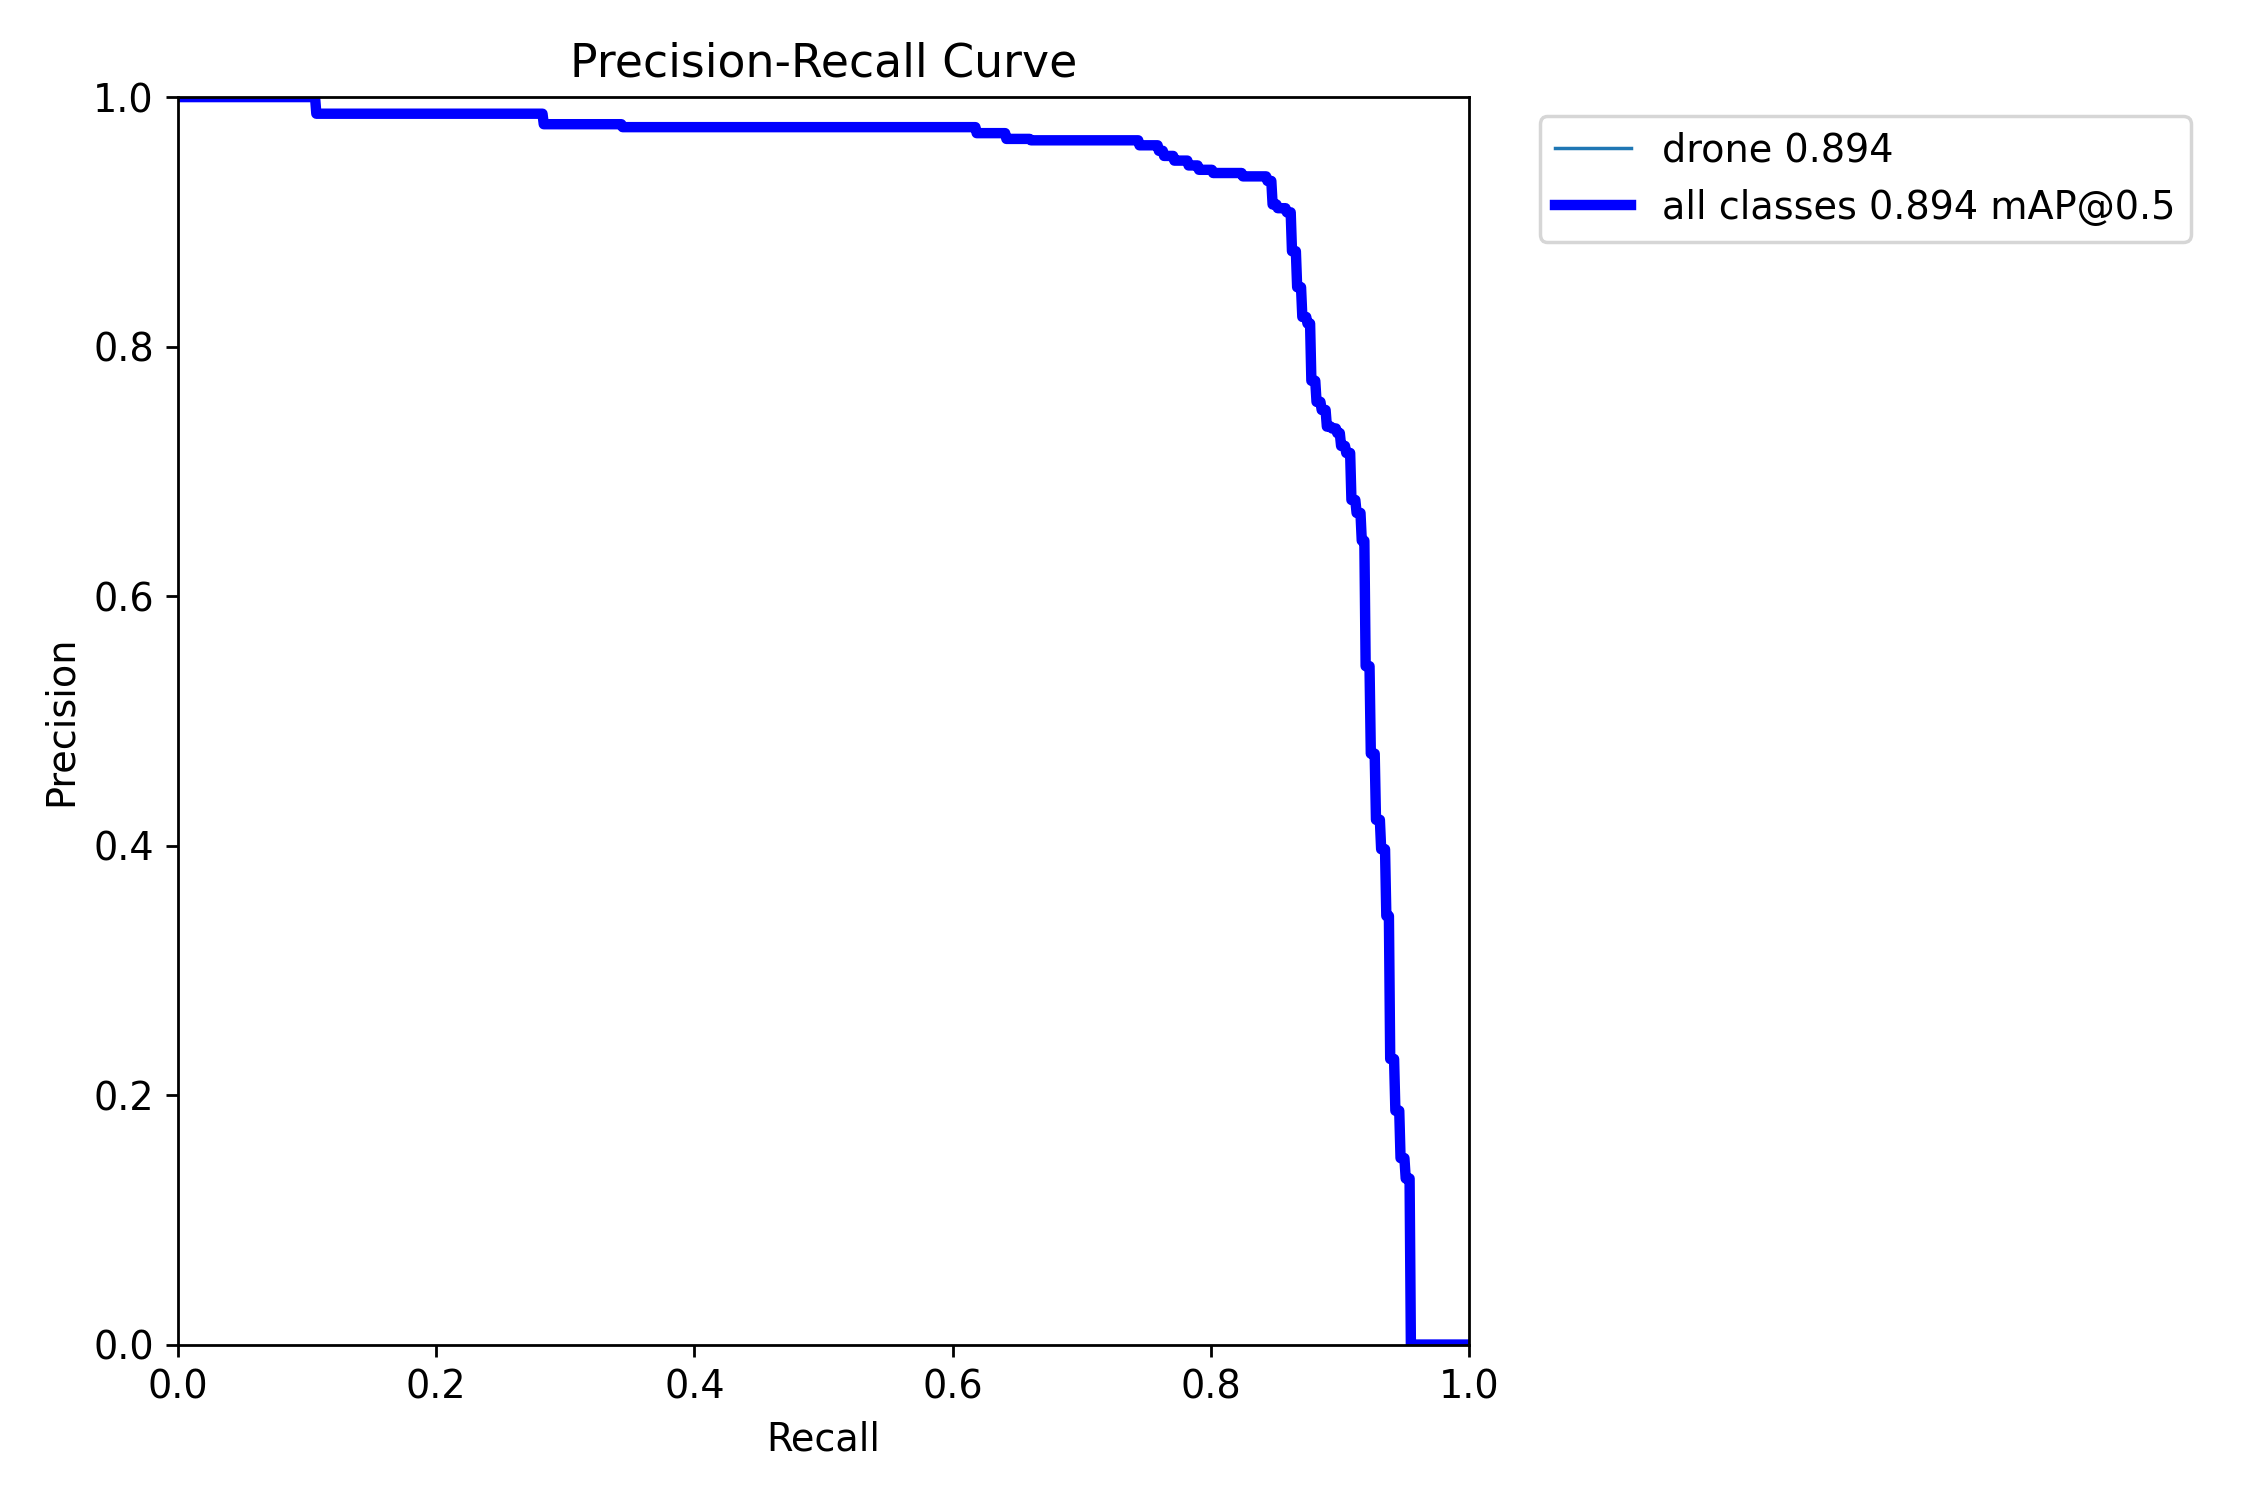
\includegraphics[width=0.78\linewidth]{figures/yolo/BoxPR_curve.png}
\caption{验证集 Precision--Recall 曲线}
\label{fig:yolopr}
\end{figure}

\subsection{多目标跟踪}

\code{MultiTracker} 支持两种工作模式，以适应不同的依赖条件：

\begin{enumerate}
  \item \term{ultralytics 内置跟踪}（推荐）：调用模型的跟踪接口并启用持久化与 ByteTrack 配置，由 ultralytics 完成 Kalman 预测与数据关联，直接返回稳定的跟踪 ID；\code{update_from_ultralytics()} 解析该结果并写入 \code{Track}。
  \item \term{独立 IOU 跟踪}（降级）：当内置跟踪不可用（未返回 ID 或未安装跟踪依赖）时，用贪心 IoU 匹配把当前帧检测关联到已有轨迹，IoU 低于阈值（默认 0.3）则新建轨迹。
\end{enumerate}

\code{Track} 对象同时保存 2D 与 3D 两条历史：\code{positions_2d}/\code{timestamps} 记录每帧的像素中心与时间，\code{positions}/\code{timestamps_3d} 只记录三角测量成功的点。两者分开保存的原因很关键：双目匹配并非每帧都成功，若把 3D 点按索引与 2D 时间戳对齐，会造成时间错位；因此 3D 点自带时间戳，写盘时以 \code{timestamps_3d} 为准。

轨迹的生命周期由三个参数控制：\code{max_missed_frames}（默认 30）决定连续多少帧未更新后判定丢失，\code{min_hits}（默认 3）决定累计命中多少次后才对外可见，从而抑制单帧误检产生的“幽灵轨迹”。

\subsection{双目三角测量}

\subsubsection{几何原理}

双目相机水平放置、光轴平行（或已知会聚角）时，同一目标在左右目图像上的横坐标差（视差）与深度成反比，如图~\ref{fig:stereo} 所示。

\begin{figure}[H]
\centering
\begin{tikzpicture}[x=1cm,y=1cm,font=\small]
% ---- 相机 ----
\draw[fill=cA, draw=cLine, rounded corners=1pt] (-0.45,-0.30) rectangle (0.45,0.30);
\draw[fill=cA, draw=cLine, rounded corners=1pt] (6.15,-0.30) rectangle (7.05,0.30);
\node[font=\scriptsize] at (0,0) {左目};
\node[font=\scriptsize] at (6.6,0) {右目};
% ---- 基线 ----
\draw[{Stealth[length=2mm]}-{Stealth[length=2mm]}, cLine] (0.45,-0.95) -- (6.15,-0.95);
\node[font=\scriptsize, fill=white, inner sep=1pt] at (3.3,-0.95) {基线 $B$};
% ---- 目标 ----
\coordinate (P) at (2.6,-4.5);
\node[circle, fill=cC, draw=cLine, inner sep=1.6pt] at (P) {};
\node[font=\scriptsize, anchor=west] at (2.78,-4.5) {目标 $P\;(x,y,z)$};
% ---- 视线 ----
\draw[cLine!70] (0,0.30) -- (P);
\draw[cLine!70] (6.6,0.30) -- (P);
% ---- 深度 ----
\draw[dashed, cLine] (2.6,-0.95) -- (2.6,-4.42);
\draw[{Stealth[length=2mm]}-{Stealth[length=2mm]}, cLine] (2.6,-1.15) -- (2.6,-4.28);
\node[font=\scriptsize, fill=white, inner sep=1pt, anchor=west] at (2.72,-2.9) {深度 $Z=\dfrac{f_xB}{d}$};
% ---- 直角标记 ----
\draw[cLine] (2.6,-1.15) -- (2.75,-1.15) -- (2.75,-1.30);
% ---- 说明 ----
\node[draw=cLine, dashed, rounded corners=2pt, fill=cD, align=left, font=\scriptsize, anchor=north west]
  at (-1.2,-5.55) {左、右目成像中目标的横坐标之差即视差 $d=x_l-x_r$，\\ 深度与视差成反比：视差越大，目标越近。};
\end{tikzpicture}
\caption{双目三角测量几何关系}
\label{fig:stereo}
\end{figure}

\subsubsection{焦距与主点}

若配置给出了像素焦距则直接使用；否则由视场角与分辨率推算：
\begin{equation}
f_x=\frac{W}{2\tan\left(\mathrm{FOV}_h/2\right)},\qquad
f_y=\frac{H}{2\tan\left(\mathrm{FOV}_v/2\right)}
\end{equation}
主点取图像中心 $(c_x,c_y)=(W/2,\,H/2)$，这是“无畸变标定信息时的合理假设”，工程上可通过标定文件替换。

\subsubsection{三角测量公式}

对左右目匹配框的中心点 $(x_l,y_l)$、$(x_r,y_r)$，视差 $d=x_l-x_r$，则
\begin{equation}
Z=\frac{f_x B}{d}
\end{equation}
\begin{equation}
X=\frac{(x_l-c_x)\,Z}{f_x}-\frac{B}{2},\qquad
Y=\frac{\left(\dfrac{y_l+y_r}{2}-c_y\right)Z}{f_y}
\end{equation}
其中 $B$ 为基线距离。$Y$ 取左右目纵坐标均值，可减小未完全行对齐带来的误差。输出坐标系为 OpenCV 相机系：$X$ 向右、$Y$ 向下、$Z$ 向前，原点位于双目光心中点。

\subsubsection{有效性校验}

三角测量前有三道校验：视差必须至少 1 像素且不小于由最大深度反推的下限；解算深度须落在 $[0.5\,\mathrm{m},\,2000\,\mathrm{m}]$；若深度超过由最小视差反推的上限，同样判为无效。任一校验失败返回 \code{None}，由调用方跳过该目标，绝不产生“无穷远”的异常点。

\subsection{跨目匹配}

左右目检测结果需要正确配对才能测距。\code{match_detections()} 采用“约束过滤 + 综合评分 + 贪心选择”的三段式策略。

\begin{enumerate}
  \item \term{硬约束}（不满足直接排除）：类别一致；垂直偏差 $|y_l-y_r|<50$ px；视差为正且在 $[d_{\min},d_{\max}]$ 内；左右框面积比不超过 2.0。
  \item \term{评分}（越小越好）：
  \begin{equation}
  s=\underbrace{|y_l-y_r|}_{\text{对齐误差}}
   +\underbrace{20\cdot\frac{|d-d_{\text{exp}}|}{d_{\text{exp}}}}_{\text{视差偏离}}
   +\underbrace{50\,(r_A-1)}_{\text{尺寸偏差}}
  \end{equation}
  其中 $d_{\text{exp}}$ 为视差范围中值，$r_A=\max(A_l,A_r)/\min(A_l,A_r)$ 为面积比。
  \item \term{类别加权}：若配置了目标类别，命中类别的得分乘以 0.5，非目标类别乘以 2.0，使无人机优先于飞鸟、飞机被配对。
\end{enumerate}

每个左目目标独立挑选得分最低且未被占用的右目目标（贪心），时间复杂度 $O(n^2)$；在单帧目标数通常小于 20 的场景下开销可忽略。

\subsection{世界坐标变换}

三角测量得到的是相机系坐标，尚需转换到统一世界系（$X$ 右、$Y$ 上、$Z$ 前），才能与其它平台的数据融合。变换按“翻转 $\rightarrow$ 偏航 $\rightarrow$ 俯仰 $\rightarrow$ 横滚 $\rightarrow$ 平移”的顺序执行：

\begin{equation}
\begin{aligned}
&\text{翻转：} && y \leftarrow -y\\
&\text{偏航 } \psi\text{：} && x' = x\cos\psi + z\sin\psi,\quad z' = z\cos\psi - x\sin\psi\\
&\text{俯仰 } \theta\text{：} && y' = y\cos\theta + z\sin\theta,\quad z' = z\cos\theta - y\sin\theta\\
&\text{横滚 } \phi\text{：} && x'' = x\cos\phi + y\sin\phi,\quad y'' = -x\sin\phi + y\cos\phi\\
&\text{平移：} && p_w = p'' + (p_x,p_y,p_z)
\end{aligned}
\end{equation}

该顺序等价于外旋（extrinsic）欧拉角 $R=R_z(\phi)R_x(\theta)R_y(\psi)$，与航空惯导的“偏航—俯仰—横滚”习惯一致。横滚的正方向做了特殊处理：绕 $Z$ 轴的正向旋转会使 $Y$ 轴倒向 $-X$（即左滚），因此右滚取 $-R_z(\phi)$。

\begin{notebox}[坐标约定提示]
配置中的 \code{pos_x/pos_y/pos_z} 是平台在世界系中的位置（米），\code{pitch/yaw/roll} 是平台朝向（度）。若平台安装方向与默认不一致，只需修改这六个参数，无需改代码。
\end{notebox}

\subsection{检测会话与并发模型}

一次检测任务对应一个 \code{DetectionSession} 对象，其状态迁移已在第~\ref{fig:sessstate} 节给出。会话的并发模型如下：

\begin{itemize}
  \item 每个会话拥有独立的后台守护线程，线程函数为 \code{_run_detection_pipeline()}；
  \item 主线程（Flask 请求线程）只负责创建会话、置位/清除事件标志、读取进度与预览帧，不参与计算；
  \item 进度、帧号、目标数、3D 点数等字段由工作线程写入、请求线程读取，均为单值写入，无需加锁；
  \item 预览帧以 JPEG 字节串缓存，接口 \code{/api/detection/preview} 直接返回，避免每次请求都重新编码；
  \item 会话注册表 \code{_sessions} 与“当前活跃会话”由 \code{_sessions_lock} 保护，防止并发创建/删除。
\end{itemize}

流水线的每个循环都执行“停止检查 $\rightarrow$ 暂停等待 $\rightarrow$ 取帧 $\rightarrow$ 检测 $\rightarrow$ 跟踪 $\rightarrow$ 匹配 $\rightarrow$ 三角测量 $\rightarrow$ 变换 $\rightarrow$ 关联”的固定序列，逻辑集中、便于定位问题。异常被捕获后写入 \code{error_message}，会话进入 \code{error} 状态而不是静默退出。

\subsection{数据桥接与落盘}

\code{tracks_to_dat()} 负责把内存中的多条轨迹合并成一个文件：

\begin{enumerate}
  \item 遍历所有 \code{Track}，收集 $(t,x,y,z)$ 四元组，时间戳取 \code{timestamps_3d}；
  \item 若没有任何 3D 点（双目全程未匹配成功），退化为写入 2D 像素坐标并将高度置 0，保证“至少有数据可回放”；
  \item 按时间排序后保存为 \file{.npz}（\code{positions}+\code{timestamps}）；
  \item 写入前调用 \code{backup_existing_fact()} 备份将被覆盖的文件，备份目录名带平台中文名，便于用户辨识；
  \item 删除同名旧 \file{.dat} 文件，避免两种格式并存导致读取歧义；
  \item 调用 \code{notify_reconstruction()} 向 5000 端口发送刷新请求，失败则静默忽略。
\end{enumerate}

\subsection{前端界面}

检测模块包含三个页面：检测工作台（视频上传、预览、控制、实时信息）、检测设置（模型与参数）、检测历史（文件与备份列表）。页面脚本分为 \file{detection.js}（接口通信封装）、\file{recognition.js}（工作台控制器）、\file{settings.js}、\file{history.js} 四个模块，通信层与界面层分离，便于替换界面而不改动接口逻辑。

工作台采用“双路上传 + 双路预览”布局：左右目各一个拖拽区，支持文件、流地址与摄像头 ID 三种输入；预览区并排显示两路带检测框的画面，右侧面板实时刷新状态、进度、目标数、3D 点数与已用时。
